\documentclass[twoside]{book}

% Packages required by doxygen
\usepackage{fixltx2e}
\usepackage{calc}
\usepackage{doxygen}
\usepackage[export]{adjustbox} % also loads graphicx
\usepackage{graphicx}
\usepackage[utf8]{inputenc}
\usepackage{makeidx}
\usepackage{multicol}
\usepackage{multirow}
\PassOptionsToPackage{warn}{textcomp}
\usepackage{textcomp}
\usepackage[nointegrals]{wasysym}
\usepackage[table]{xcolor}

% Font selection
\usepackage[T1]{fontenc}
\usepackage[scaled=.90]{helvet}
\usepackage{courier}
\usepackage{amssymb}
\usepackage{sectsty}
\renewcommand{\familydefault}{\sfdefault}
\allsectionsfont{%
  \fontseries{bc}\selectfont%
  \color{darkgray}%
}
\renewcommand{\DoxyLabelFont}{%
  \fontseries{bc}\selectfont%
  \color{darkgray}%
}
\newcommand{\+}{\discretionary{\mbox{\scriptsize$\hookleftarrow$}}{}{}}

% Page & text layout
\usepackage{geometry}
\geometry{%
  a4paper,%
  top=2.5cm,%
  bottom=2.5cm,%
  left=2.5cm,%
  right=2.5cm%
}
\tolerance=750
\hfuzz=15pt
\hbadness=750
\setlength{\emergencystretch}{15pt}
\setlength{\parindent}{0cm}
\setlength{\parskip}{3ex plus 2ex minus 2ex}
\makeatletter
\renewcommand{\paragraph}{%
  \@startsection{paragraph}{4}{0ex}{-1.0ex}{1.0ex}{%
    \normalfont\normalsize\bfseries\SS@parafont%
  }%
}
\renewcommand{\subparagraph}{%
  \@startsection{subparagraph}{5}{0ex}{-1.0ex}{1.0ex}{%
    \normalfont\normalsize\bfseries\SS@subparafont%
  }%
}
\makeatother

% Headers & footers
\usepackage{fancyhdr}
\pagestyle{fancyplain}
\fancyhead[LE]{\fancyplain{}{\bfseries\thepage}}
\fancyhead[CE]{\fancyplain{}{}}
\fancyhead[RE]{\fancyplain{}{\bfseries\leftmark}}
\fancyhead[LO]{\fancyplain{}{\bfseries\rightmark}}
\fancyhead[CO]{\fancyplain{}{}}
\fancyhead[RO]{\fancyplain{}{\bfseries\thepage}}
\fancyfoot[LE]{\fancyplain{}{}}
\fancyfoot[CE]{\fancyplain{}{}}
\fancyfoot[RE]{\fancyplain{}{\bfseries\scriptsize Generated by Doxygen }}
\fancyfoot[LO]{\fancyplain{}{\bfseries\scriptsize Generated by Doxygen }}
\fancyfoot[CO]{\fancyplain{}{}}
\fancyfoot[RO]{\fancyplain{}{}}
\renewcommand{\footrulewidth}{0.4pt}
\renewcommand{\chaptermark}[1]{%
  \markboth{#1}{}%
}
\renewcommand{\sectionmark}[1]{%
  \markright{\thesection\ #1}%
}

% Indices & bibliography
\usepackage{natbib}
\usepackage[titles]{tocloft}
\setcounter{tocdepth}{3}
\setcounter{secnumdepth}{5}
\makeindex

% Hyperlinks (required, but should be loaded last)
\usepackage{ifpdf}
\ifpdf
  \usepackage[pdftex,pagebackref=true]{hyperref}
\else
  \usepackage[ps2pdf,pagebackref=true]{hyperref}
\fi
\hypersetup{%
  colorlinks=true,%
  linkcolor=blue,%
  citecolor=blue,%
  unicode%
}

% Custom commands
\newcommand{\clearemptydoublepage}{%
  \newpage{\pagestyle{empty}\cleardoublepage}%
}

\usepackage{caption}
\captionsetup{labelsep=space,justification=centering,font={bf},singlelinecheck=off,skip=4pt,position=top}

%===== C O N T E N T S =====

\begin{document}

% Titlepage & ToC
\hypersetup{pageanchor=false,
             bookmarksnumbered=true,
             pdfencoding=unicode
            }
\pagenumbering{roman}
\begin{titlepage}
\vspace*{7cm}
\begin{center}%
{\Large My Project }\\
\vspace*{1cm}
{\large Generated by Doxygen 1.8.11}\\
\end{center}
\end{titlepage}
\clearemptydoublepage
\tableofcontents
\clearemptydoublepage
\pagenumbering{arabic}
\hypersetup{pageanchor=true}

%--- Begin generated contents ---
\chapter{Hierarchical Index}
\section{Class Hierarchy}
This inheritance list is sorted roughly, but not completely, alphabetically\+:\begin{DoxyCompactList}
\item \contentsline{section}{App\+Delegate()}{\pageref{category_app_delegate_07_08}}{}
\item $<$U\+I\+Application\+Delegate$>$\begin{DoxyCompactList}
\item \contentsline{section}{App\+Delegate}{\pageref{interface_app_delegate}}{}
\end{DoxyCompactList}
\item U\+I\+Responder\begin{DoxyCompactList}
\item \contentsline{section}{App\+Delegate}{\pageref{interface_app_delegate}}{}
\end{DoxyCompactList}
\end{DoxyCompactList}

\chapter{Class Index}
\section{Class List}
Here are the classes, structs, unions and interfaces with brief descriptions\+:\begin{DoxyCompactList}
\item\contentsline{section}{\hyperlink{interface_app_delegate}{App\+Delegate} }{\pageref{interface_app_delegate}}{}
\item\contentsline{section}{\hyperlink{category_app_delegate_07_08}{App\+Delegate()} }{\pageref{category_app_delegate_07_08}}{}
\item\contentsline{section}{\hyperlink{interface_camera}{Camera} }{\pageref{interface_camera}}{}
\item\contentsline{section}{\hyperlink{interface_cube}{Cube} }{\pageref{interface_cube}}{}
\item\contentsline{section}{\hyperlink{interface_entity}{Entity} }{\pageref{interface_entity}}{}
\item\contentsline{section}{\hyperlink{interface_entity_render}{Entity\+Render} }{\pageref{interface_entity_render}}{}
\item\contentsline{section}{\hyperlink{interface_entity_shader_manager}{Entity\+Shader\+Manager} }{\pageref{interface_entity_shader_manager}}{}
\item\contentsline{section}{\hyperlink{interface_game_engine_tests}{Game\+Engine\+Tests} }{\pageref{interface_game_engine_tests}}{}
\item\contentsline{section}{\hyperlink{interface_game_view_controller}{Game\+View\+Controller} }{\pageref{interface_game_view_controller}}{}
\item\contentsline{section}{\hyperlink{category_game_view_controller_07_08}{Game\+View\+Controller()} }{\pageref{category_game_view_controller_07_08}}{}
\item\contentsline{section}{\hyperlink{interface_g_l_s_l_utils}{G\+L\+S\+L\+Utils} }{\pageref{interface_g_l_s_l_utils}}{}
\item\contentsline{section}{\hyperlink{protocol_i_shape-p}{$<$\+I\+Shape$>$} }{\pageref{protocol_i_shape-p}}{}
\item\contentsline{section}{\hyperlink{interface_loader}{Loader} }{\pageref{interface_loader}}{}
\item\contentsline{section}{\hyperlink{interface_load_utils}{Load\+Utils} }{\pageref{interface_load_utils}}{}
\item\contentsline{section}{\hyperlink{interface_master_render}{Master\+Render} }{\pageref{interface_master_render}}{}
\item\contentsline{section}{\hyperlink{interface_model_texture}{Model\+Texture} }{\pageref{interface_model_texture}}{}
\item\contentsline{section}{\hyperlink{interface_raw_model}{Raw\+Model} }{\pageref{interface_raw_model}}{}
\item\contentsline{section}{\hyperlink{interface_shader_manager}{Shader\+Manager} }{\pageref{interface_shader_manager}}{}
\item\contentsline{section}{\hyperlink{interface_shader_program}{Shader\+Program} }{\pageref{interface_shader_program}}{}
\item\contentsline{section}{\hyperlink{interface_sky_box}{Sky\+Box} }{\pageref{interface_sky_box}}{}
\item\contentsline{section}{\hyperlink{interface_sky_box_shape}{Sky\+Box\+Shape} }{\pageref{interface_sky_box_shape}}{}
\item\contentsline{section}{\hyperlink{interface_terrain}{Terrain} }{\pageref{interface_terrain}}{}
\item\contentsline{section}{\hyperlink{interface_terrain_shape}{Terrain\+Shape} }{\pageref{interface_terrain_shape}}{}
\item\contentsline{section}{\hyperlink{interface_terrain_textures_pack}{Terrain\+Textures\+Pack} }{\pageref{interface_terrain_textures_pack}}{}
\item\contentsline{section}{\hyperlink{interface_textured_model}{Textured\+Model} }{\pageref{interface_textured_model}}{}
\item\contentsline{section}{\hyperlink{interface_vector2f}{Vector2f} }{\pageref{interface_vector2f}}{}
\item\contentsline{section}{\hyperlink{interface_vector3f}{Vector3f} }{\pageref{interface_vector3f}}{}
\end{DoxyCompactList}

\chapter{Class Documentation}
\hypertarget{interface_app_delegate}{}\section{App\+Delegate Class Reference}
\label{interface_app_delegate}\index{App\+Delegate@{App\+Delegate}}
Inheritance diagram for App\+Delegate\+:\begin{figure}[H]
\begin{center}
\leavevmode
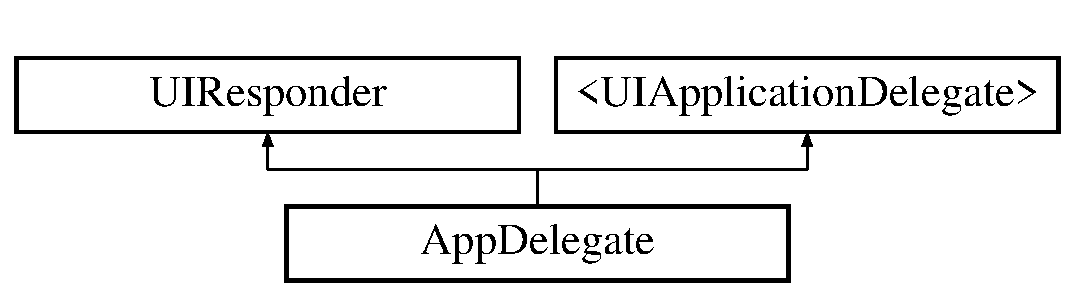
\includegraphics[height=2.000000cm]{interface_app_delegate}
\end{center}
\end{figure}
\subsection*{Properties}
\begin{DoxyCompactItemize}
\item 
U\+I\+Window $\ast$ {\bfseries window}\hypertarget{interface_app_delegate_acf48ac24125e688cac1a85445cd7fac2}{}\label{interface_app_delegate_acf48ac24125e688cac1a85445cd7fac2}

\end{DoxyCompactItemize}


The documentation for this class was generated from the following file\+:\begin{DoxyCompactItemize}
\item 
Game\+Engine/App\+Delegate.\+h\end{DoxyCompactItemize}

\hypertarget{category_app_delegate_07_08}{}\section{App\+Delegate() Category Reference}
\label{category_app_delegate_07_08}\index{App\+Delegate()@{App\+Delegate()}}


The documentation for this category was generated from the following file\+:\begin{DoxyCompactItemize}
\item 
Game\+Engine/App\+Delegate.\+m\end{DoxyCompactItemize}

%--- End generated contents ---

% Index
\backmatter
\newpage
\phantomsection
\clearemptydoublepage
\addcontentsline{toc}{chapter}{Index}
\printindex

\end{document}
